\documentclass[../practica.root.tex]{subfiles}

\begin{document}

\setcounter{section}{0}
\section{Vectores, Rectas y Planos}

\begin{enumerate}
    \item[5.] Graficar en el plano el conjunto \( \S = \left\{ (x,y)\in\R^2 / \left\|(x,y)\right\| = 1 \right\} \)
    
    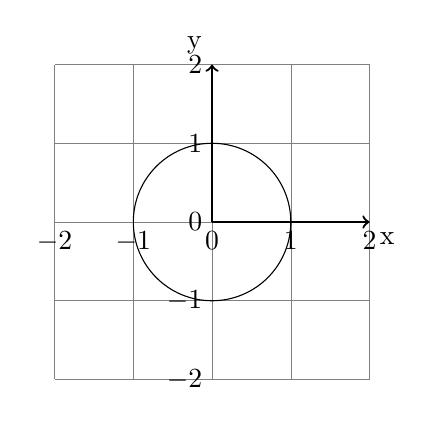
\begin{tikzpicture}
        \draw[very thin,gray] (-2,-2) grid (2,2);
        \draw[thick,->] (0,0) -- (2,0) node[anchor=north west] {x};
        \draw[thick,->] (0,0) -- (0,2) node[anchor=south east] {y};
        \foreach \x in {-2,-1,0,1,2}
            \draw (\x,0) node[anchor=north] {$\x$};
        \foreach \y in {-2,-1,0,1,2}
            \draw (0,\y) node[anchor=east] {$\y$};
        \draw (0,0) circle(1);
    \end{tikzpicture}
    \item[6.] Determinar todos los valores de \(k\) tale que:
    \begin{enumerate}
        \item \( \| A \| = 2 \) si \( A = (1,k,0) \)
        \[ \sqrt{A_x^2 + A_y^2 + A_z^2} = 2 \]
        \[ \sqrt{1^2 + k^2 + 0^2} = 2 \]
        \[ \sqrt{1 + k^2} = 2 \]
        \[ (1 + k^2) = 2^2 \]
        \[ k^2 = 3 \]
        \[ k = \sqrt{3} \lor k = -\sqrt{3} \]
        \item \( d(A,B) = 2 \) si \( A = (1,1,1) \) y \( B = (k,-k,2) \)
        \[ \| A - B \| = 2 \]
        \[ \| (1,1,1) - (k,-k,2) \| = 2 \]
        \[ \| (1-k,1+k,-1) \| = 2 \]
        \[ \sqrt{(1-k)^2 + (1+k)^2 + 1} = 2 \]
        \[ \sqrt{1-2k+k^2 + 1+2k+k^2 + 1} = 2 \]
        \[ \sqrt{2k^2+3} = 2 \]
        \[ 2k^2+3 = 2^2 \]
        \[ 2k^2 = 4-3 \]
        \[ k^2 = \frac{1}{2} \]
        \[ k = \pm\sqrt{\frac{1}{2}} = \pm\frac{1}{\sqrt{2}} = \pm\frac{1}{\sqrt{2}}\cdot\frac{\sqrt{2}}{\sqrt{2}} = \pm\frac{\sqrt{2}}{2} \]
        \[ k = \frac{\sqrt{2}}{2} \lor k = -\frac{\sqrt{2}}{2} \]
        \item \( \| A \| = 1 \) si \( A = k(2,2,1) \)
        \[ A = k(2,2,1) = (2k,2k,k) \]
        \[ \| A \| = 1 \]
        \[ \| (2k,2k,k) \| = 1 \]
        \[ \sqrt{(2k)^2 + (2k)^2 + k^2} = 1 \]
        \[ \sqrt{4k^2 + 4k^2 + k^2} = 1 \]
        \[ \sqrt{9k^2} = \sqrt{9}\cdot\sqrt{k^2} = 1 \]
        \[ 3\|k\| = 1 \]
        \[ \|k\| = \frac{1}{3} \]
        \[ k = \pm\frac{1}{3} \]
        \[ k = \frac{1}{3} \lor k = -\frac{1}{3} \]
    \end{enumerate} 
    \item[11.] Encontrar todos los vectores ortogonales a:
    \begin{enumerate}
        \item[\textcolor{red}{\blacksquare}] \( A = (1,2) \)
        \[ A\cdot\vec{v} = 0 \]
        \[ (1, 2)\cdot(x, y) = 0 \]
        \[ x + 2y = 0 \]
        \[ x = -2y \]
        \[ (x, y) = (-2y, y) = \boxed{y(-2,1)} \]
        \item[\textcolor{green}{\blacksquare}] \( E_1 = (1,0) \)
        \[ E_1\cdot\vec{v} = 0 \]
        \[ (1, 0)\cdot(x, y) = 0 \]
        \[ x = 0 \]
        \[ (x, y) = (0, y) = \boxed{y(0, 1)} \]
        \item[\textcolor{blue}{\blacksquare}] \( E_2 = (0,1) \)
        \[ E_2\cdot\vec{v} = 0 \]
        \[ (0, 1)\cdot(x, y) = 0 \]
        \[ y = 0 \]
        \[ (x, y) = (x, 0) = \boxed{x(1, 0)} \]
    \end{enumerate}
    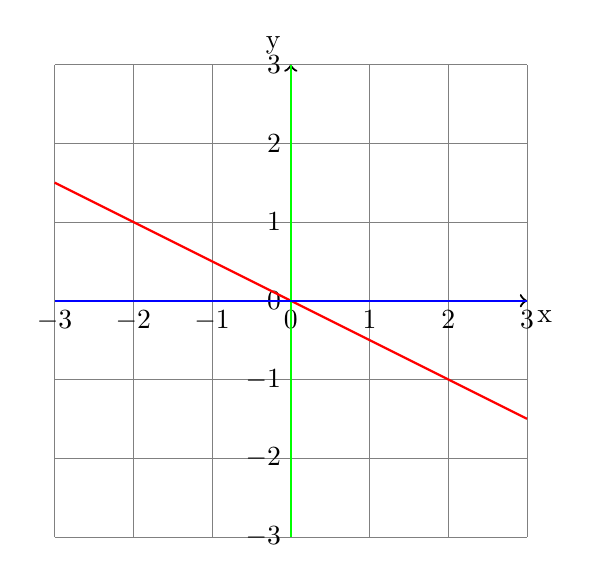
\begin{tikzpicture}
        \coordinate (O) at (0,0);
        \coordinate (BL) at (-3,-3);
        \coordinate (TR) at (3,3);
        \draw[very thin,gray] (BL) grid (TR);
        \draw[thick,->] (O) -- (O -| TR) node[anchor=north west] {x};
        \draw[thick,->] (O) -- (O |- TR) node[anchor=south east] {y};
        \foreach \x in {-3,-2,-1,0,1,2,3}
            \draw (\x,0) node[anchor=north] {$\x$};
        \foreach \y in {-3,-2,-1,0,1,2,3}
            \draw (0,\y) node[anchor=east] {$\y$};
        % A
        \draw[thick,red] (-3,1.5) -- (3,-1.5);
        % E_1
        \draw[thick,green] (0,3) -- (0,-3);
        % E_2
        \draw[thick,blue] (3,0) -- (-3,0);
    \end{tikzpicture}
    \begin{enumerate}
        \item \( E_1 = (1,0,0) \)
        \[ E_1\cdot\vec{v} = 0 \]
        \[ (1,0,0)\cdot(x,y,z) = 0 \]
        \[ x = 0 \]
        \[ (x,y,z) = (0,y,z) = (0,y,0) + (0,0,z) = \boxed{y(0,1,0) + z(0,0,1)} \]
        \item \( E_2 = (0,1,0) \)
        \[ E_2\cdot\vec{v} = 0 \]
        \[ (0,1,0)\cdot(x,y,z) = 0 \]
        \[ y = 0 \]
        \[ (x,y,z) = (x,0,z) = \boxed{x(1,0,0) + z(0,0,1)} \]
        \item \( E_3 = (0,0,1) \)
        \[ E_3\cdot\vec{v} = 0 \]
        \[ (0,0,1)\cdot(x,y,z) = 0 \]
        \[ z = 0 \]
        \[ (x,y,z) = (x,y,0) = \boxed{x(1,0,0) + y(0,1,0)} \]
        \item \(E_1\) y \(E_2\)
        \[ E_1\x E_2 = (0,0,1) \]
        \[ \boxed{k(0,0,1), k \in \R} \]
        \item \(E_1\) y \(E_3\)
        \[ E_1\x E_3 = (0,-1,0) \]
        \[ \boxed{k(0,-1,0), k \in \R} \]
        \item \(E_2\) y \(E_3\)
        \[ E_2\x E_3 = (1,0,0) \]
        \[ \boxed{k(1,0,0), k \in \R} \]
    \end{enumerate}
    \item[] 
\end{enumerate}
\end{document}